%% -*- Latex -*- 
%% 
%% app_1.tex - appendix on differential geometry
%% 

\chapter{Differential Geometry}
\label{app:differential-geometry}


The curves discussion in the following take a mathematical geometric
viewpoint to explain the theory needed to develop a tool for analyzing
the line skeleton. Also presented is the mathematical foundation used
in the discussion of the deformable model description found in later
chapters. As a result the coverage of the mathematical theory will
include the basic definitions of curve analysis and differential
geometry along with the needed analysis methods needed. Normally texts
will treat the two-dimensional curves, also referred to as plane
curves, but here only space curves are considered.

As presented here the theory is derived from several sources which
have different mathematical nomenclature. The nomenclature is sought
to be consistent throughout the report; references may use another
nomenclature.

\section{Space Curve}
\label{sec:space-curve}

With a Cartesian coordinate system being given, a space curve $C$ is
represented by
\begin{equation}
  \label{eq:space-curve}
  \bm{r}(t) = [x(t),y(t),z(t)] =   x(t)\hat{\mathbf{x}} + y(t)\hat{\mathbf{y}} + z(t)\hat{\mathbf{z}}.
\end{equation}
This representation is called a parametric representation of the curve
$C$ with $t$ as the parameter. An arc of a curve is the part of the
curve between any two points of the curve, and an arc is also in
itself a curve. The curves of the vascular skeleton is approximated by
straight lines.

\section{Velocity and Acceleration}
\label{sec:velocity-acceleration}

The tangent vector to a curve $C$ at $r(t)$ is given
\begin{equation}
  \label{tangent-vector}
  v(t) = r'(t) = \frac{dr}{dt}(t)
\end{equation}
by showing that
\begin{equation}
  \nonumber
  r'(t_0) = \lim_{t\rightarrow t_0} \frac{r(t) - r(t_0)}{t - t_0}
\end{equation}
The unit tangent vector is given
\begin{equation}
  \label{eq:unit-tangent-vector}
  \mathbf{u}(t) = \frac{1}{\lvert r'(t)\rvert}r'(t)
\end{equation}
as it points in the direction of the tangent and has unit length.

The vector $v$ or $r'$ is the tangent to $C$ and has the length
\begin{equation}
  \label{eq:velocity}
  \lvert v\rvert = \sqrt{r' \cdot r'} = \frac{ds}{dt}
\end{equation}
where $s$ is the arc length. Here $\frac{ds}{dt}$ is the speed of $C$
at the point $t$, and the vector $v$ is called the velocity vector.



The derivative of the velocity vector is the acceleration vector and
is denoted $a$
\begin{equation}
  \label{eq:acceleration}
  a(t) = v'(t) = r''(t)
\end{equation}


\section{Arc Length}
\label{sec:arc-length}

The curve $C$ is parametrized by $t$ and the arclength $s$ of a curve
$C$, which is the length along the curve, is then given by
\begin{equation}
  \nonumber
  s = \int_a^b ds = \int_a^b \frac{ds}{dt}dt = \int_a^b \lvert r'(t)\rvert dt
    = \int_a^b \sqrt{r'(t)\cdot r'(t)} \,dt
\end{equation}
by observing that $\frac{ds}{dt}$ is the magnitude of the velocity
with which the end of the radius vector $r$ moves. It gives that
$\frac{ds}{dt}$ is equal to the magnitude of the derivative of $r(t)$.
For the space curve $C$ given by Eq.~(\ref{eq:space-curve}) the arc
length is
\begin{equation}
  \label{eq:arclength}
  s = \int_a^b \sqrt{{x'}^2(t)+{y'}^2(t)+{z'}^2(t)} \,dt
\end{equation}

\section{Curvature}
\label{sec:curvature}

The simplest form of curvature is encountered in calculus and is
called extrinsic curvature. Another type, intrinsic curvature for
surfaces, is not discussed further here. The curvature $\kappa (s)$ of a
curve $C$ is represented by $r(s)$ where the arclength $s$ as
parameter
\begin{equation}
  \label{curvature-s-parameter}
  \kappa (s) = \frac{\lvert r'(s) \times r''(s) \rvert}{\lvert r'(s) \rvert^3}
\end{equation}
It is assumed that $r''$ exists as $r$ must be twice differentiable
for the curvature $\kappa$ to exist.  Since $\kappa$ is the length of
the rate of change of the unit tangent vector of $C$ with $s$,
$\kappa$ measures the deviation of $C$ from the tangent at each point
of $C$.

If the curvature is not equal to zero ($\kappa > 0$) then the unit
vector $\mathbf{p}(s)$ in the direction of $\mathbf{u}'(s)$ is
\begin{equation}
  \label{eq:unit-principal-vector}
  \mathbf{p} = \frac{1}{\kappa}\mathbf{u}'
\end{equation}
and the vector is called the unit principal normal vector.

The vector $\mathbf{b}$ 
\begin{equation}
  \label{eq:unit-binormal-vector}
  \mathbf{b} = \mathbf{u} \times \mathbf{p}
\end{equation}
is called the unit binormal vector of the curve $C$. 

\section{Torsion}
\label{sec:torsion}

The torsion is the rate of change of the osculating plane of a space
curve. The torsion $\tau$ is positive for a right-handed curve and
negative for a left-handed curve. A curve with curvature not equal to
zero is planar if torsion is equal to zero. Torsion is defined by
\begin{equation}
  \label{eq:torsion}
  \tau(s) = -\mathbf{p}(s) \cdot \mathbf{b}'(s)
\end{equation}
and also
\begin{equation}
  \label{eq:real-torsion}
  \tau(s) = \frac{[r'(s),r''(s),r'''(s)]}{\lvert r'(s) \times r''(s) \rvert^2}
\end{equation}
and is a scalar value just as the curvature is a scalar value. By
introducing the torsion $\tau (s)$ of a curve $C$ the derivative
$\mathbf{b}' = \frac{d\mathbf{b}}{ds}$ of the unit binormal vector is
used. It is assumed that $r(s)$ is three times differentiable so
$\mathbf{b}'$ exist. It can be shown that $\mathbf{b}'$ and
$\mathbf{u}$ are perpendicular and that $\mathbf{b}' = \alpha
\mathbf{p}$, where $\alpha$ is customary set to $-\tau$.

\section{Frenet Frame and Natural Equations}
\label{sec:frenet-frame-natural-equations}

Curves of 2~space and 3~space can be described by Frenet formulas
(also known as Serret-Frenet formulas) which consist of vector
differential equations which can be related to the properties of a
parametrized curve.  From the definition of
Eq.~(\ref{eq:unit-tangent-vector}), (\ref{eq:unit-principal-vector}),
and~(\ref{eq:unit-binormal-vector}) if can be seen that the vectors
$\mathbf{u}$, $\mathbf{p}$, and $\mathbf{b}$ constitutes a
right-handed triple of unit vectors. The triple is called a trihedron
and can be seen on figure~\ref{fig:trihedron}. The point $t$ on the
curve $C$ is the point of consideration for which the three vectors
are valid.

The set of vectors, $\mathbf{u}$, $\mathbf{p}$, and $\mathbf{b}$, are
linearly independent. Any vector in space may be represented through a
combination of these vectors. When the derivatives of the vectors
exists they are referred to as the Frenet formulas. Written on matrix form
the Frenet formulas are given
\begin{equation}
  \label{eq:frenet-matrix}
  \begin{bmatrix}
    \mathbf{u}' \\
    \mathbf{p}' \\
    \mathbf{b}'
  \end{bmatrix}
  =
  \begin{bmatrix}
    0       & \kappa   & 0       \\
    -\kappa & 0        & \tau    \\
    0       & -\tau    & 0 
  \end{bmatrix}
  \begin{bmatrix}
    \mathbf{u} \\
    \mathbf{p} \\
    \mathbf{b}
  \end{bmatrix}
\end{equation}
The three straight lines through that point in the directions of $u$,
$p$, $b$ are called the tangent, the principal normal, and the
binormal of $C$ and figure~\ref{fig:trihedron} shows the names of the
three planes spanned by each pair of those curves.  A space curve is
uniquely determined (except for the geometric position in space) by
its curvature $\kappa$ and torsion $\tau$ as continuous functions of
arc length $s$ (see figure~\ref{fig:frenet-frame}). The equations
$\kappa = \kappa(s)$ and $\tau = \tau(s)$ are called the natural
equations of a space curve, which show why they are basic in the
differential geometry of space curves.  The curvature $\kappa(s)$ of a
curve $C$, represented by $r(s)$ with arc length $s$ as parameter, is
defined by
\begin{equation}
  \kappa(s) = \lvert u'(s)\rvert = \lvert r''(s)\rvert
\end{equation}
Here $u(s) = r'(s)$ is the unit tangent vector of $C$, and we have to
assume that $r(s)$ is twice differentiable, so that $r''(s)$ exists.

\begin{figure}[htbp]
  \centering
  \psfrag{tangent}{tangent $\mathbf{u}(s)$}
  \psfrag{binormal}{binormal $\mathbf{b}(s)$}
  \psfrag{principal normal}{principal normal $\mathbf{p}(s)$}
  \psfrag{curve}{curve $r(s)$}
  \psfrag{normal plane}{normal plane}
  \psfrag{rectifying plane}{rectifying plane}
  \psfrag{osculating plane}{osculating plane}
  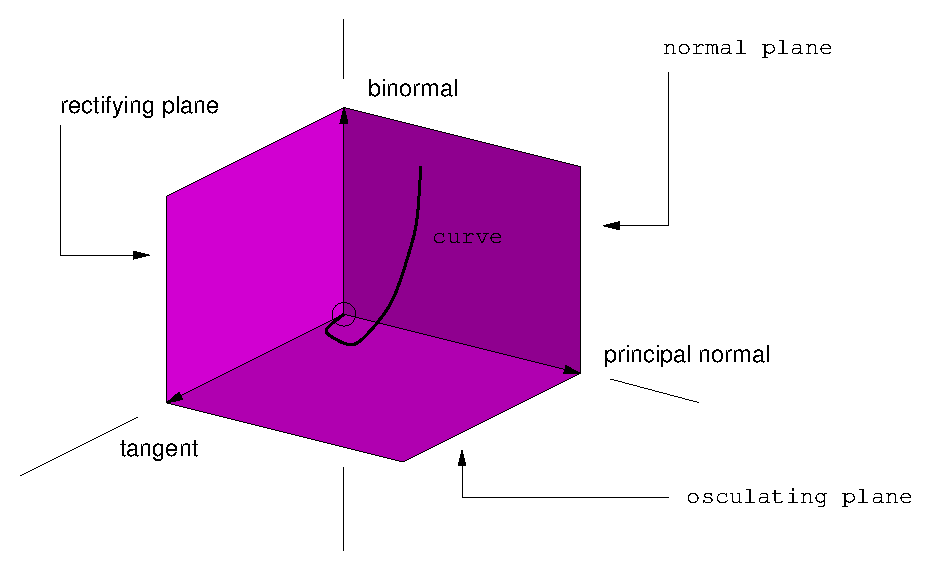
\includegraphics{curvature-trihedron.eps}
  \caption{Explanation of the Frenet frame and its vectors and planes.}
  \label{fig:trihedron}
\end{figure}

\begin{figure}[htbp]
  \centering
  \psfrag{osculating circle}{osculating circle}
  \psfrag{r(s)}{$r(s)$}
  \psfrag{curvature}{$\kappa(s)$}
  \psfrag{p(s)}{$\mathbf{p}(s)$}
  \psfrag{u(s)}{$\mathbf{u}(s)$}
  \psfrag{b(s)}{$\mathbf{b}(s)$}
  \psfrag{tau}{$\tau(s)$}
  \psfrag{cur}{$\kappa(s)$}
  \psfrag{x}{$x$}
  \psfrag{y}{$y$}
  \psfrag{z}{$z$}
  \mbox{%
    \subfigure[Top of the curve $r(s)$ and the corresponding
    osculating circle]{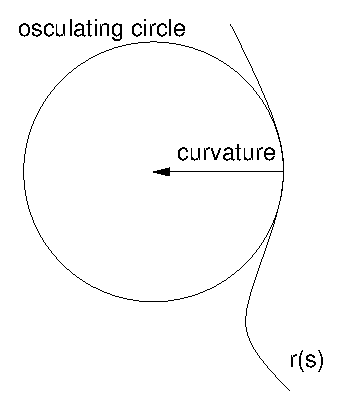
\includegraphics[scale=0.8]{frenet-plane.eps}}\quad
    \subfigure[Frenet frame with the three perpendicular frame unit
    vectors imposed on the curve and osculating with indication of the
    torsion and curvature measures]{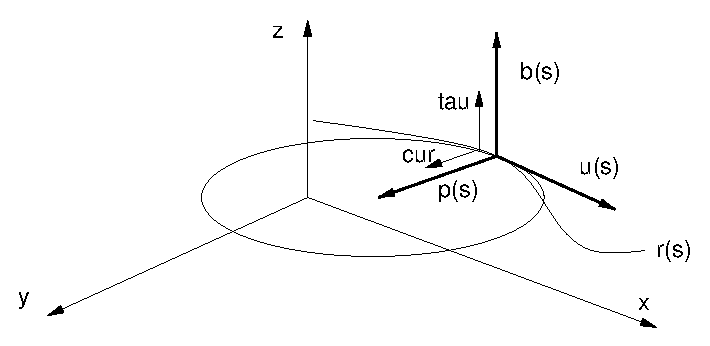
\includegraphics[scale=0.8]{frenet-plane-frame.eps}}}
  \caption{The Frenet frame with torsion and curvature illustrated.}
  \label{fig:frenet-frame}
\end{figure}

\section{Summary}
\label{sec:summary}

Examination and calculation of the curvature and torsion of a curve,
involves the three vectors (tangent, principal normal and binormal)
forming the Frenet frame. The tangent vector $T$ is a unit vector in
the directorion of the velocity $V$. The other vectors usually defined
in terms of the arc length parameter $s$
\begin{eqnarray}
  \text{Tangent } \mathbf{u}(s) &=& \frac{r'(s)}{\lvert r'(s) \rvert} \\
  \text{Principal normal } \mathbf{p}(s) &=& \frac{r''(s) - \lvert r'(s) \rvert \mathbf{u}(s)}{\left\lvert r''(s) - \lvert r'(s) \rvert \mathbf{u}(s) \right\rvert} \\
  \text{Binormal } \mathbf{b}(s) &=& \mathbf{p}(s) \times \mathbf{u}(s) \\
  \text{Curvature } \kappa(s) &=& \frac{\lvert r'(s) \times r''(s) \rvert}{\lvert r'(s) \rvert^3} \\
  \text{Torsion } \tau(s) &=& \frac{[r'(s),r''(s),r'''(s)]}{\lvert r'(s) \times r''(s) \rvert^2}
\end{eqnarray}
Usually curves are given in terms of parameters other than arc
length. Still the formulas can be used but for some other parameter
$t$. $\frac{d}{ds}=\frac{1}{v}\frac{d}{dt}$ by the Chain Rule where
$v=\frac{ds}{dt}=\lvert V\rvert$ is the speed. An alternative set of
formulas lead to less complicated calculations:
\begin{eqnarray}
  V \times A &=& v^3\kappa V \\
  \mathbf{u} &=& \mathbf{b} \times \mathbf{p} \\
  \tau &=& \frac{(V \times A) \frac{dA}{dt}}{\lvert V \times A\rvert^2}
\end{eqnarray}
An osculating circle at a point $r(t)$ on the curve is a circle that
best approximates the curve near $r(t)$, which has the same tangent,
principal normal, and curvature as the curve. The radius of this
circle is $1 / \kappa(t)$ and its center lies at that distance from
$r(t)$ in the direction of $\mathbf{u}(t)$ (at $r(t) +
\mathbf{u}(t)/\kappa(t)$). The circle lies in the osculating plane
determined by the vectors $\mathbf{p}(t)$ and $\mathbf{u}(t)$, so it
has the parametric representation
\begin{equation}
  r(t) + \frac{(1 + cos(s))\mathbf{u}(t) +
    sin(s)\mathbf{p}(t)}{\kappa(t)}, 
  \quad 0 \leq s \leq 2\pi
\end{equation}

\clearemptydoublepage

%%% Local Variables: 
%%% mode: latex
%%% mode: reftex
%%% mode: flyspell
%%% TeX-master: "master"
%%% End: 
